\section{Avaliação}

As seções a seguir descrevem a metodologia utilizada para compreender as implicações do uso da abordagem proposta na identificação de conflitos semânticos. Além disso, verificamos o quão perto as nossas implementações atuais da análise estão perto de uma implementação ideal de OA. Fazemos também uma breve comparação do desempenho das implementações. Por fim, apresentamos os resultados obtidos e às ameaças a validade.

\subsection{Dataset}
Para avaliar a capacidade da análise proposta de detectar interferência entre as contribuições de diferentes versões, foi utilizado um conjunto de dados com 78 cenários de integração de projetos \emph{open-source} Java extraídos do \emph{Github}. \rev{Cada um desses cenários contém um método ou campo de uma classe modificado em ambas versões Left e Right --- isto é, os ramos integrados em uma determinada operação de merge.} Esse tipo de cenário em específico foi escolhido, pois, são mais suscetíveis a ocorrência de interferência. Alguns desses cenários foram aproveitados de outros trabalhos relacionados, sendo 5 de Da Silva et. al. \cite{LeusonSilva2020}, 19 de Barros Filho  \cite{InformationFlowRoberto}, 26 de De Souza et. al. \cite{10.1145/958160.958177} e 7 de Cavalcanti et. al. \cite{10.1109/ASE.2019.00097}. Os outros 21 cenários foram minerados a partir de uma lista de projetos \emph{open-source} populares utilizando o \emph{miningframework}. \rev{A lista com todos os cenários e projetos utilizados pode ser encontrada no Apêndice online \rev{\cite{sitesbes2022}}.}

O processo de coleta dos dados utilizados é ilustrado pela \hyperref[fig:mineracao]{Figura 8}. A ferramenta de mineração recebe como entrada um arquivo com uma lista de repositórios no \emph{Github} e cria \emph{forks} dos repositórios para configurar uma ferramenta de CI (Integração Contínua). Logo após o \emph{miningframework} cria o cenário contendo os arquivos das versões \emph{Base}, \emph{Left} e \emph{Right} que serão utilizados para coletar as linhas modificadas por cada um dos desenvolvedores. Em seguida, a ferramenta executa o processo descrito na caixa tracejada para cada um dos \emph{commits} de \emph{merge} envolvido no \emph{three-way merge}\footnote{Um  \emph{three-way merge} acontece quando dois conjuntos de alterações em um arquivo base são integrados à medida que são aplicados, em vez de aplicar um e, em seguida, integrar o resultado com o outro.} dos projetos passados como entrada. 

\begin{figure}[!h]
    \centering
    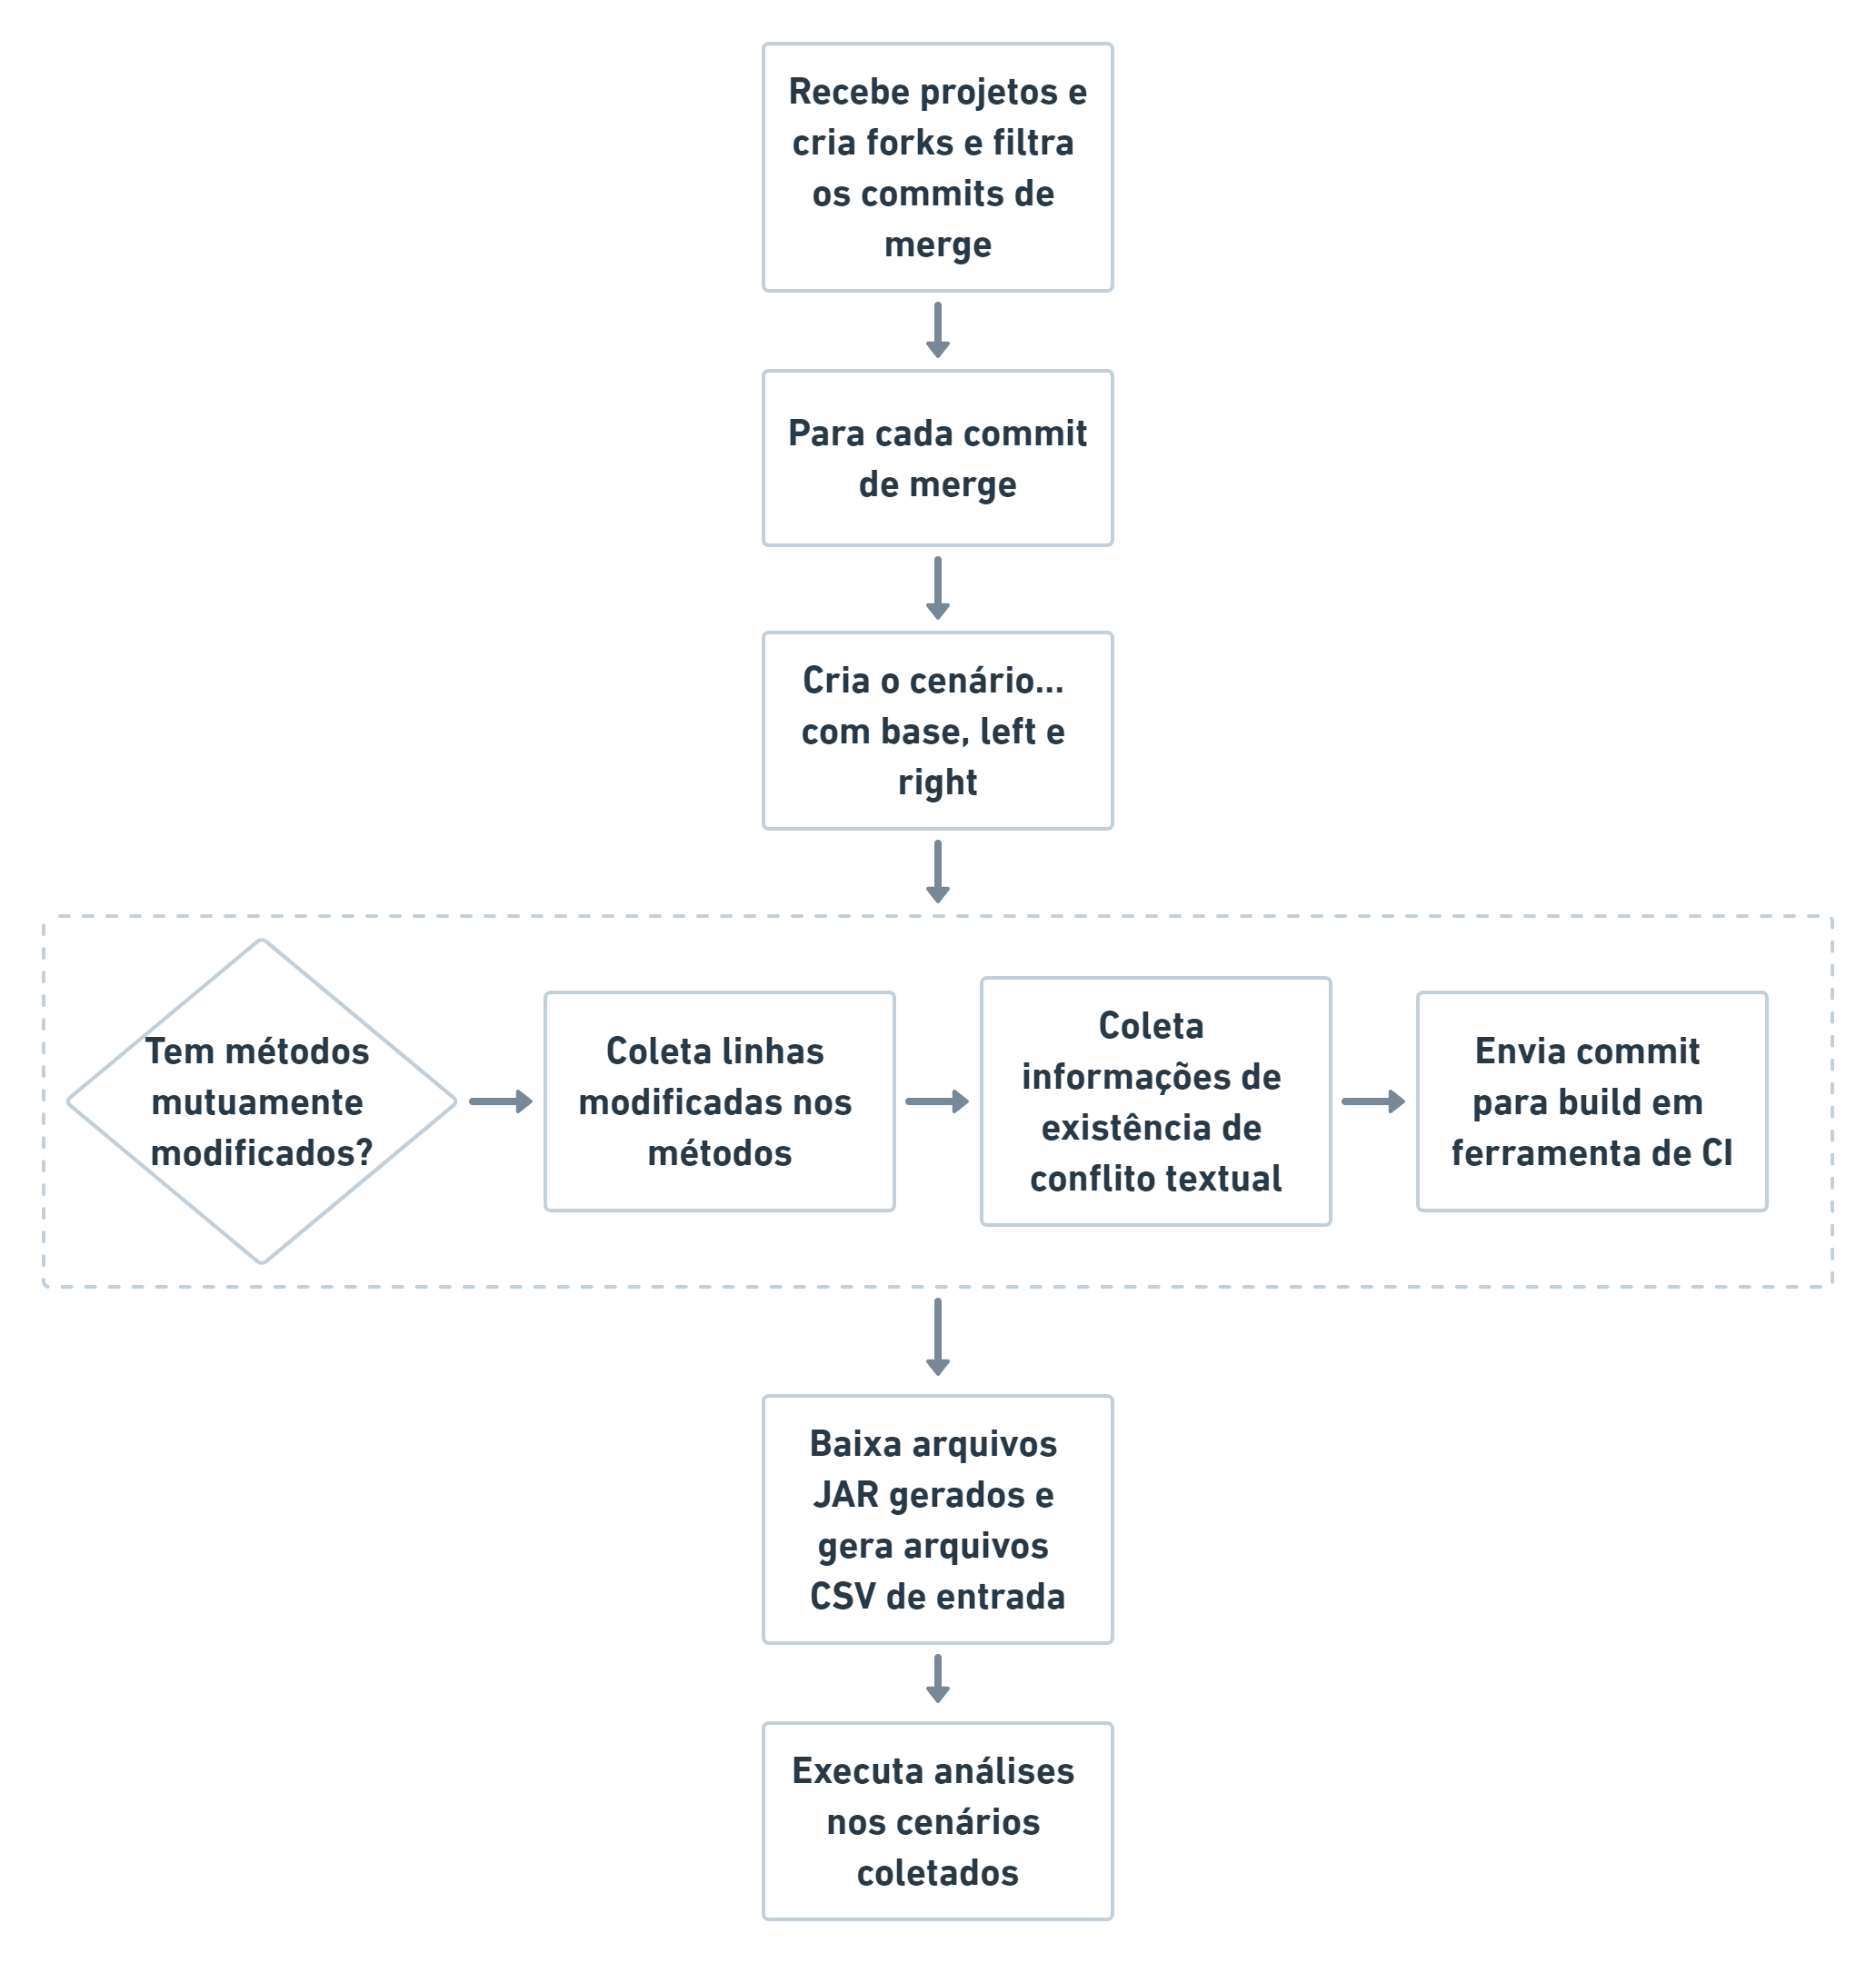
\includegraphics[width=0.8\linewidth]{samples/images/Fluxo de mineracao.png}
    \caption{Fluxo de coleta dos dados sobre os cenários de integração}
    \label{fig:mineracao}
\end{figure}

Para cada \emph{commit}, a ferramenta primeiro checa se existem métodos ou atributos de classe modificados por ambas as versões \emph{Left} e \emph{Right}, caso não existam, o \emph{commit} é ignorado. Caso existam, a ferramenta continua o processo de coleta de dados, coleta os números das linhas das modificações de \emph{Left} e \emph{Right}, faz o replay do \emph{merge} e depois verifica a existência de conflitos de integração textuais e registra em uma planilha. Por fim, envia o cenário para geração dos arquivos \emph{JAR} em uma ferramenta de CI. A ferramenta gera um arquivo de configuração para a plataforma de CI \emph{Github Actions}\footnote{Um exemplo de arquivo gerado para um projeto real (jsoup) pode ser visto em: https://gist.github.com/barbosamaatheus/073dc8caa24e3e775e2483629c476856.
}, que usa os sistemas de \emph{build} \emph{Maven} ou \emph{Gradle} para gerar os arquivos JAR.


O Processo supracitado foi utilizado na maioria dos casos, no entanto, em alguns desses cenários, o mapeamento das linhas do código-fonte, extraídos a partir do \emph{bytecode}, pode ser impreciso, por isso precisaram passar por adaptações, assim dizemos que eles são realistas. Esse problema ocorre principalmente nos casos em que há chamadas de método encadeadas que ocupam várias linhas. Isso está ligado ao modo como a associação do número da linha é armazenada no arquivo de classe (\emph{.class}) e no histórico do compilador \emph{javac}. Para evitar esses comandos que ocupam várias linhas, quebramos o mesmo em vários comandos que ocupam apenas uma linha, através de simples refatorações de extração de variáveis no código-fonte do projeto para que o comportamento original do programa fosse preservado, mas que o \emph{bytecode} tivesse o mapeamento esperado das linhas. Esse tratamento foi aplicado em três cenários.

Para a análise de cenários cujo método de entrada tinha pelo menos um argumento com tipo não primitivo, adicionamos um método que instancia os parâmetros e chama o método de entrada. Essa estratégia foi aplicada em quatro cenários e usada apenas pela implementação \emph{intraprocedural} e foi necessária, pois a análise não reconhece parâmetros de tipos não primitivos que não foram instanciados previamente no código. 

Após executar o processo descrito anteriormente, para cada um dos \emph{commits} de \emph{merge}, a ferramenta baixa os arquivos \emph{JAR} gerados na plataforma de CI e gera os arquivos de entrada para a execução da análise de OA.

Todos os arquivos utilizados para avaliação, assim como as instruções para gerar os arquivos \emph{JAR} que foram gerados manualmente podem ser encontrados no projeto \href{https://github.com/spgroup/mergedataset}{mergedataset}\footnote{Este repositório agrupa um conjunto de cenários de mesclagem com conflitos semânticos conhecidos, coletados de estudos relacionados. https://github.com/spgroup/mergedataset}. Um resumo da amostra utilizada pode ser observada no Apêndice Online \rev{\cite{sitesbes2022}}.

\subsection{Metodologia}
\label{sec:metodologia}

A \hyperref[fig:fluxo-execucao]{Figura 9} apresenta o fluxo de trabalho seguido no estudo empírico.

\begin{figure}[!h]
    \centering
    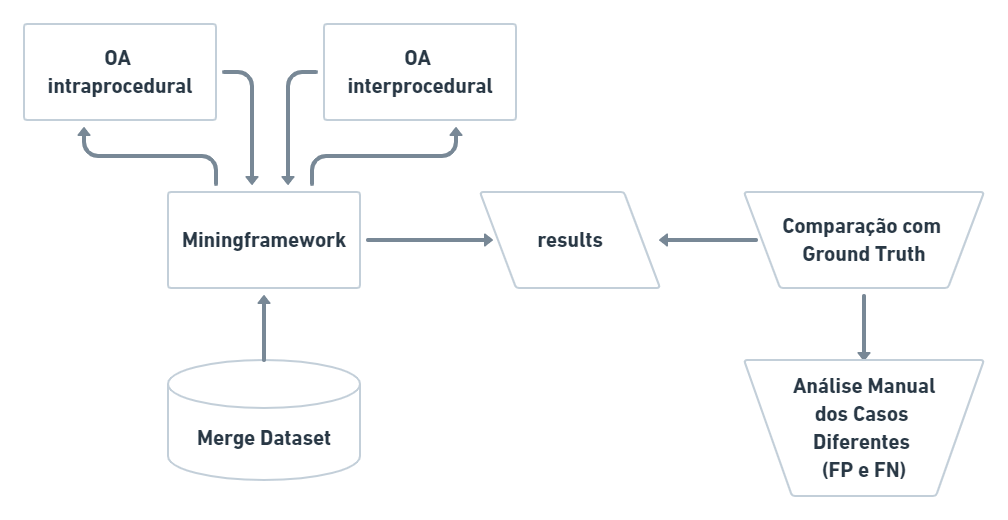
\includegraphics[width=0.8\linewidth]{images/Fluxo da avaliação.png}
    \caption{Fluxo da execução da avaliação das análises.}
    \label{fig:fluxo-execucao}
\end{figure}


Com os dados necessários para os 78 cenários, o \href{https://github.com/spgroup/miningframework}{miningframework} foi utilizado para executar as implementações  \emph{intraprocedural} e  \emph{interprocedural} em cada um dos cenários. Para fins de avaliação, o resultado de uma análise é considerado positivo para um cenário específico se a execução retornar uma ou mais interferências.

Todos os 78 cenários do conjunto de dados também foram analisados manualmente, utilizando o protocolo disponível no Apêndice Online \rev{\cite{sitesbes2022}}, de modo a verificar a existência de interferências entre as modificações de \emph{Left} e \emph{Right}, e assim estabelecer um \emph{Ground Truth}. Para definição do \emph{Ground Truth}, foi usado um processo estruturado de checagem dupla, onde cada cenário foi atribuído a dois colaboradores que realizaram a análise de forma individual registrando justificativas para suas decisões. A análise individual dos dois colaboradores foi comparada e caso o resultado convergisse, o mesmo seria adotado com \emph{Ground Truth} do cenário. Em caso de divergência, os colaboradores se reuniam e discutiam o cenário, buscando chegar a um consenso. Nos casos em que o consenso não foi atingido, o cenário era apresentado a outro colaborador que juntos, tomavam a decisão.

Buscando verificar a capacidade da análise em detectar interferência entre as contribuições ou até mesmo compor uma ferramenta para detecção de conflitos de integração semânticos mais robusta, os resultados apresentados pelas implementações da análise proposta foram comparados com o \emph{Ground Truth} em cada cenário. Adicionalmente, para verificarmos o quão próximo a nossa implementação atual está de uma implementação ideal de OA, comparamos o resultado da ferramenta com \emph{Ground Truth} exclusivo de OA. 

Por fim, foi realizada uma análise manual dos casos diferentes (Falsos Positivos e Falsos Negativos) onde foi possível identificar os motivos pelos quais a análise não produziu o resultado esperado.\footnote{Feita apenas para a abordagem \emph{interprocedural}} Isso não é o objetivo principal deste trabalho, assim como a otimização da implementação e a avaliação da métrica de tempo. Desta forma, não aprofundamos esses itens, mas pretendemos realizar em trabalhos futuros, assim como a análise dos casos positivos, onde verificaremos se os alertas gerados pela análise correspondem às interferências detectadas na análise manual.

\subsection{Resultados}

\subsubsection{Resultados Reportados nas Execuções das Implementações da Analíse}

Ao executar a abordagem \emph{intraprocedural} da análise proposta para 78 cenários do \emph{dataset} obtivemos 13,2\% de casos reportados como verdadeiros, ou seja, a análise reportou pelo menos uma interferência nesses cenários. Em 80,9\% dos casos, a análise não detectou nenhuma interferência. Ainda foram reportados 4 casos (5,9\%) que não foram encontrados pela análise, isso ocorreu, pois, esses cenários tinham apenas remoções de linhas feitas pelo desenvolvedor \emph{Right}. Outros 10 casos apresentaram erro na execução. Os casos com erro ou que não foram encontrados foram desconsiderados para fins de comparação com o \emph{ground truth}.

Já a execução \emph{interprocedural} também reportou os mesmos 4 casos (5,1\%) como não encontrado. Além disso, apresentou 6 casos (7,7\%) em que a análise foi interrompida por exceder o limite de tempo\footnote{O  \emph{timeout} pode acontecer, pois, devido à característica da abordagem \emph{interprocedural} que acessa e analisa o corpo de todos os métodos chamados nós próprios métodos analisados, o que exige um tempo maior de execução por isso é definido um tempo limite que quando é atingido, para a execução da análise e retorna um status de \emph{timeout}.} estipulado para cada cenário. Esses 10 casos, foram desconsiderados para fins de comparação com o \emph{ground truth}. A execução \emph{interprocedural} também reportou 15.4\% dos casos como verdadeiros e 71,8\% como falso.

\subsubsection{OA x Análise Manual de LOI}

Os resultados apresentados nessa subseção foram obtidos comparando os resultados da execução das implementações da análise proposta com o \emph{Ground Truth} para interferência localmente observável. Essa comparação pretende avaliar o algoritmo para detecção de interferências entre as contribuições das versões integradas, portanto, para detecção de conflitos semânticos.

\begin{figure}[!h]
    \centering
    \includegraphics[width=0.9\linewidth]{images/OA x Análise Manual de LOI.png}
    \caption{Resultados da análise em comparação com o \emph{Ground Truth} de LOI.}
    \label{fig:loi-x-groundtruthloi}
\end{figure}

Os resultados ilustrados na \hyperref[fig:loi-x-groundtruthloi]{Figura 10} mostram a comparação dos 64 cenários considerados na execução \emph{intraprocedural} com o \emph{ground truth} de LOI. Obteve-se uma taxa alta de 34,4\% de falsos negativos e 7,8\% de falsos positivos. Logicamente, os outros 57,9\% foram de acertos da ferramente, sendo 51,6\% verdadeiros negativos e 6,3\% de verdadeiros positivos. 

Ainda na \hyperref[fig:loi-x-groundtruthloi]{Figura 10}, conseguimos observar também os resultados da comparação dos 68 cenários considerados na execução \emph{interprocedural} com o \emph{ground truth} de LOI. Obtendo-se uma taxa de 27,9\% de falsos negativos e 7,4\% de falsos positivos. os outros 64,7\% foram de acertos da ferramente, sendo 54,4\% verdadeiros negativos e 10,3\% de verdadeiros positivos.

A \hyperref[tab:erros-inter-loi]{Tabela 1} apresenta um sumário com a descrição e a quantidade de erros da análise \emph{interprocedural} proposta.

\begin{table}[h]
    \centering
    \begin{tabularx}{\linewidth}{X c c}
        \hline
        Descrição do Cenário (em relação à causa do erro) & \multicolumn{1}{l}{Quantidade} & \multicolumn{1}{l}{Tipo de erro} \\ \hline
        String com mais de uma linha é alterada em linhas diferentes & 1 & FN \\ \hline
        Alterações apenas na inicialização de atributos que possuem mais de uma linha & 2 & FN \\ \hline
        \emph{Callgraph} não consegue encontrar possíveis classes de destino, pois faltam dependências & 2  & FN \\ \hline
        Interferência não é detectável com OA & 14 & FN \\ \hline
        Não existe interferência entre as contribuições & 5  & FP\\ \hline
    \end{tabularx}
    \caption{Descrições dos cenários em que a análise \emph{interprocedural} proposta errou na detecção de LOI.}
    \label{tab:erros-inter-loi}
\end{table}

Os dois últimos itens da tabela já são esperados, pois, a análise foi projetada para detectar OA e como já dito anteriormente a existência de OA não implica necessariamente na existência de LOI e vice-versa.

O primeiro caso da tabela pode ser observado na imagem ilustrada na \hyperref[fig:ad2be67]{Figura 11}. Para esse caso temos que \emph{Left} e \emph{Right} alteraram a \emph{String} que vai ser usado no retorno da função. O \emph{ground truth} classifica isso como OA, no entanto, ao nível de execução da implementação da análise, o \emph{Soot framework} vai gerar variáveis temporárias para cada uma das linhas, dessa forma a análise não consegue associar as mudanças feitas pelos desenvolvedores a mesma variável. Isso é uma limitação da implementação que pretendemos resolver em trabalhos futuros.

\begin{figure}[h]
    \begin{lstlisting}[escapechar=!]
    @Override
    public String toString()() {
        return "KafkaSpoutConfig{" +
        ", k!\colorbox{yellow}{eys" + getK}!eyDeserializer!\colorbox{yellow}{() +}!
        ", value=" + !\colorbox{yellow}{getV}!alueDeserializer!\colorbox{yellow}{()}! +
       ...
        !\colorbox{green}{   }!
        ...
        '}';
    }
    \end{lstlisting}
    \caption{\rev{Cenário Storm ad2be67 no método toString() como exemplo para o falso negativo.}}
    \label{fig:ad2be67}
    \centering
\end{figure}

A partir dos resultados das execuções das implementações da análise foram calculadas as métricas representadas pela \hyperref[tab:metrics-loi]{Tabela 2}.

Para a métrica de precisão, a análise \emph{interprocedural} obteve o valor de 0,6, enquanto a análise \emph{intraprocedural} proposta tem uma precisão de 0,4. Os valores são bem próximos e indicam que alguns dos casos indicados como positivos foram classificados corretamente, mas também que grande parte dos casos indicados como positivos foram classificados incorretamente. A quantidade de falsos positivos é esperada, pois, existem casos em que existe OA,
mas \emph{Ground truth} de LOI é falso, desta forma as implementações vão detectar OA, mas não existe interferência real. Um exemplo disso acontece um dos desenvolvedores fez apenas uma refatoração estrutural no código.

Para a métrica de revocação, a análise \emph{interprocedural} obteve o valor de 0,3, enquanto a análise \emph{intraprocedural} obteve 0,2. Novamente os valores são muito próximos e indicam que a maioria dos casos positivos não são detectados pelas abordagens. A priori, esses números podem parecer baixos, no entanto, a principal razão para isso está em nossa amostra que contém diversos tipos de interferência, como, por exemplo, casos em que um desenvolvedor escreve em uma variável que outro desenvolvedor futuramente lê. Esses tipos diferentes de interferência não são detectados pelo algoritmo de OA que busca apenas variáveis atribuídas por dois desenvolvedores diferentes. A combinação da análise de OA com outras análises melhoraria consideravelmente os resultados de revocação. Além disso, a solução dos problemas e limitações conhecidas nas implementações atuais, colocaria os resultados de revocação em seu nível máximo. 

A análise \emph{interprocedural}, por sua característica e natureza, tem uma acurácia melhor por ser uma análise menos sensível e detectar mais casos positivos que a análise \emph{intraprocedural}, isso fica comprovado no resultado onde a análise \emph{interprocedural} teve uma acurácia de 0,64, enquanto a \emph{intraprocedural} recebeu 0,57. De modo geral, os resultados para essa métrica são considerados bons, mas podem ser significativamente melhorados aplicando principalmente as soluções supracitadas para melhoria da revocação.

\begin{table}[!h]
    \centering
    \begin{tabular}{ l  l  l }
        \hline
                  & Intraprocedural & Interprocedural  \\
        \hline
        Precisão & 0,4 & 0,6 \\
        \hline
        Revocação & 0,2 & 0,3 \\
        \hline
        Acurácia  & 0,57 & 0,64 \\
        \hline
        
    \end{tabular}
    \caption{Resultados das Métricas para a detecção de LOI}
    \label{tab:metrics-loi}
\end{table}

Comparando os resultados das duas execuções, podemos observar resultados semelhantes com uma leve vantagem para a abordagem \emph{interprocedural}. Isso é esperado, pois a \emph{interprocedural} percorre e analisa uma quantidade maior de código-fonte, o que faz com que ela consiga sinalizar casos adicionais de interferência. No entanto, pelo mesmo motivo, o custo de execução \emph{interprocedural} é maior. Isso faz com que a abordagem \emph{intraprocedural} seja ainda mais relevante. 

Em geral, podemos concluir que a análise proposta consegue detectar interferência entre as modificações em um cenário de integração, o que pode indicar que ela é uma boa ferramenta para detecção de conflitos de integração semânticos. No entanto,  existem outros tipos de cenário de interferência que análises OA não é capaz de detectar, o que indica que somente a análise proposta não é suficiente para ser utilizada sozinha, como uma ferramenta confiável para detecção de conflitos semânticos. A análise proposta poderia ser combinada com outras análises que buscam detectar outros tipos de interferência para criar uma ferramenta mais robusta. Análises de OA podem errar na detecção de interferência e com a análise proposta não é diferente. Nesse  sentido, uma ferramenta com suporte a OA pode ser muito sensível e apresentar falsos positivos e falsos negativos.

\subsubsection{OA x Análise Manual de OA}

Os resultados apresentados nessa subseção foram obtidos comparando os resultados da análise proposta com o \emph{Ground Truth} para OA. Essa comparação visa avaliar a capacidade da análise proposta para detecção da existência de substituição de atribuições (OA) entre as contribuições de dois desenvolvedores em um cenário de integração de código. Através dessa comparação, podemos identificar a qualidade das implementações atuais e o quão perto elas estão de uma implementação ideal de OA.

A partir dos resultados obtidos através da execução das implementações da análise foram calculadas as métricas representadas pela \hyperref[tab:metrics-oa]{Tabela 3}.

\begin{table}[!h]
    \centering
    \begin{tabular}{ l  l  l }
        \hline
        & Intraprocedural & Interprocedural  \\
        \hline
        Precisão & 0,44 & 1.0 \\
        \hline
        Revocação & 0,22 & 0,6 \\
        \hline
        Acurácia  & 0,7 & 0,88 \\
        \hline
        
    \end{tabular}
    \caption{Resultados das métricas para a detecção de OA}
    \label{tab:metrics-oa}
\end{table}

A análise proposta se mostrou capaz de detectar cenários com substituições de atribuições entre as contribuições, principalmente na sua abordagem \emph{interprocedural}. No entanto, a análise reportou falsos positivos e falsos negativos. O número de falsos positivos foi baixo e isso indica que a análise reporta poucos "alarmes falsos", gerando um custo pequeno para o desenvolvedor, que não vai ser distraído facilmente por problemas que não existem de fato. Os falsos negativos estão associados a limitações da análise, e acontecem, por exemplo, quando as modificações introduzidas pelos desenvolvedores estão em inicializações de atributos com múltiplas linhas e não existe um método de entrada. 

Com isso concluímos que a análise apresentou excelentes índices, princialmente na métrica de  acurácia. (0,7\% para \emph{intraprocedural} e 0,88\% para \emph{interprocedural}). Isso significa que as implementações atuais precisam de poucos ajustes para se tornarem ideias no sentido de detecção de OA.

\subsubsection{Detalhes da execução}
Embora o desempenho não fosse uma prioridade para nosso projeto, deixamos aqui os registros dos dados coletados relacionados ao tempo de execução da análise.

As duas abordagens da análise foram executadas utilizando uma máquina virtual com sistema operacional Linux Ubuntu 20.04.2 LTS 64-bit, 4 \emph{Gigabyte} de memória RAM, processador Intel® Core™ i5-9300H CPU @ 2.40GHz × 4. Ambas tiveram o \emph{timeout} configurado em 240 segundos. A execução \emph{interprocedural} foi configurada com um limite de profundidade no acesso aos métodos de 5. 

Com dados de uma execução e tomando a média dos tempos medidos, a execução \emph{intraprocedural} levou 2,32 segundos/por cenário para analisar toda a amostra, com mediana de 1,09 e desvio padrão de 2,42.  Já a execução \emph{interprocedural} teve media de 28,12 segundos/por cenário, mediana de 3,94 e desvio padrão de 68,81.

Analisando os resultados podemos perceber que a abordagem \emph{interprocedural} é consideravelmente mais lenta em relação à média de tempo por cenário do que a abordagem \emph{intraprocedural}. Isso é esperado, pois, como a \emph{intraprocedural} tem como característica, ignorar as chamadas de método no método de entrada, ela percorre um caminho mais curto durante a execução. O contrário ocorre na execução \emph{interprocedural} que permite acessar e analisar todo o corpo de todas as chamadas de método até que o seu limite de profundidade, definido por parâmetro, seja atingido. Utilizando o referencial dos resultados atuais, indicamos a implementação \emph{interprocedural} pois a mesma obteve resultados melhores na detecção de interferência, mas devido ao seu custo maior, acreditamos que a mesma possa ser utilizada em rotinas que executam à noite, por exemplo. Para contextos onde o tempo é um fator limitante a implementação \emph{intraprocedural} é a mais recomendada. 

É importante ressaltar que as implementações utilizadas nesse trabalho são protótipos e não foram otimizadas visando desempenho, uma vez que o objetivo era verificar a capacidade da mesma em detectar interveniências. Com isso, queremos dizer que os resultados de desempenho podem ser substancialmente melhorados.  

\subsection{Ameaças a validade}

Nosso estudo se restringe à ocorrência de interferência local. Portanto, é possível que nossos exemplos tenham cenários de \emph{merge} que as alterações não interferem umas com as outras localmente, mas interferem globalmente. O contrário também pode ocorrer. Então o número de falsos negativos e falsos positivos em relação a uma noção de interferência pode diferir do nosso relatório de resultados.



Além disso, ao definir o \emph{ground truth}, conhecer os resultados da análise proposta antes da análise manual pode ter influenciado o veredicto. Por exemplo,
sabendo que a ferramenta não foi bem sucedida para um determinado cenário traz o risco de impedir uma análise manual mais aprofundada. Para reduzir essa ameaça, envolvemos dois autores na definição de \emph{ground truth}, e exigiu-se que eles fornecessem uma explicação de porque não há interferência. 

\rev{O tipo de cenário contidos no nosso dataset, com mudanças em paralelo no mesmo método ou atributo pode ser mais suscetível a ocorrência de interferência, mas isso não influencia o resultado final principal apresentado no artigo sobre a acurácia e performance de uma ferramenta baseada na análise OA, já que no dataset temos vários casos de interferência, mas também vários casos sem interferência, e nossa avaliação principal não é sobre a frequência com que interferência ocorre, mas sim se análise estática seria viável para detectar interferência. Adotamos esse critério de filtro dos cenários de merge para reduzir um pouco a dificuldade de analisar manualmente cenários reais para confirmar a ocorrência de interferência. Nenhum outro filtro sobre o conteúdo dos métodos e atributos dos cenários foi aplicado.}

O objetivo principal deste trabalho é verificar a utilidade da análise proposta em detectar interferências entre as contribuições. Com isso, não investimos na otimização das implementações da análise, o que pode fazer com que a implementação atual apresente erros. Alguns problemas conhecidos já foram mencionados, mas podem existir outros problemas que ainda não foram detectados. 
Alguns dos cenários do \emph{dataset} utilizado precisaram de adaptações realistas. Essas alterações foram realizadas no código-fonte de sete cenários buscando manter o máximo das características originais. No entanto, essas alterações foram feitas de forma manual e não foram executados testes para validar que o comportamento original foi mantido, no entanto, deixamos o alerta que esses casos são tratados como cenários realistas e não reais de fato.

